\documentclass[12pt]{article}
\usepackage[T1, T2A]{fontenc}
\usepackage[utf8]{inputenc}
\usepackage[russian]{babel}
\usepackage{hyperref}
\usepackage{graphicx}
\graphicspath{ {../Images/} }

\author{Григорий Матюхин}
\date{\today}
\title{Лабораторная работа \textnumero8.\\Планировщики событий}

\begin{document}
\maketitle
\newpage
\tableofcontents
\newpage
\section{Цель работы}
Получение навыков работы с планировщиками событий \texttt{cron} и \texttt{at}.

\section{Последовательность выполнения работы}

\subsection{Планирование задач с помощью cron}
\begin{enumerate}
	\item Запустите терминал и получите полномочия администратора:
	\item Посмотрите статус демона \texttt{crond}:
	      \\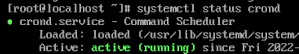
\includegraphics{1.png}
	\item Посмотрите содержимое файла конфигурации \texttt{/etc/crontab}:
	\item Посмотрите список заданий в расписании:
	      \\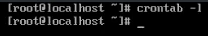
\includegraphics{2.png}
	\item Откройте файл расписания на редактирование. Добавьте следующую строку в файл расписания: \texttt{*/1 * * * * logger This message is written from root cron}:
	      \\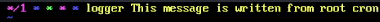
\includegraphics{3.png}
	\item Посмотрите список заданий в расписании:
	      \\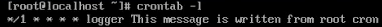
\includegraphics{4.png}
	\item Не выключая систему, через некоторое время (2–3 минуты) просмотрите журнал системных событий:
	      \\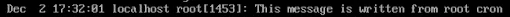
\includegraphics{5.png}
	\item Измените запись в расписании crontab на следующую \texttt{0 */1 * * 1-5 logger This message is written from root cron}:
	      \\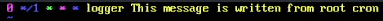
\includegraphics{6.png}
	\item Посмотрите список заданий в расписании:
	      \\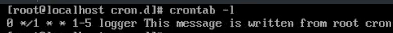
\includegraphics{7.png}
	\item Перейдите в каталог \texttt{/etc/cron.hourly} и создайте в нём файл сценария с именем \texttt{eachhour}:
	      \\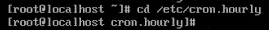
\includegraphics{8.png}
	\item Откройте файл \texttt{eachhour} для редактирования и пропишите в нём следующий скрипт (запись сообщения в системный журнал):
	      \begin{verbatim}
#!/bin/sh
logger This message is written at $(date)
        \end{verbatim}
	      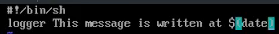
\includegraphics{9.png}
	\item Сделайте файл сценария \texttt{eachhour} исполняемым:
	      \\
\includegraphics{10.png}
	\item Теперь перейдите в каталог \texttt{/etc/crond.d} и создайте в нём файл с расписанием eachhour. Откройте этот файл для редактирования и поместите в него следующее содержимое \texttt{11 * * * * root logger This message is written from /etc/cron.d}:
	      \\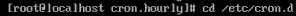
\includegraphics{11.png}
	      \\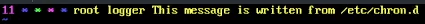
\includegraphics{12.png}
	\item Не выключая систему, через некоторое время (2–3 часа) просмотрите журнал системных событий:
	      \\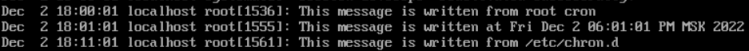
\includegraphics{13.png}

\end{enumerate}

\subsection{Планирование заданий с помощью at}
\begin{enumerate}
	\item Запустите терминал и получите полномочия администратора:
	\item Проверьте, что \texttt{служба atd} загружена и включена:
	      \\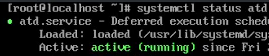
\includegraphics{14.png}
	\item Задайте выполнение команды \texttt{logger message from at} в 9:30 (или замените на любое другое время, когда вы работаете над этим упражнением). Для этого введите \texttt{at 9:30}. Затем введите \texttt{logger message from at}:
	      \\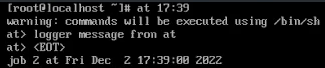
\includegraphics{15.png}
	\item Убедитесь, что задание действительно запланировано \texttt{atq}
	      \\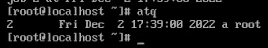
\includegraphics{16.png}
	\item Посмотрите, появилось ли соответствующее сообщение в лог-файле в указанное вами время.
	      \\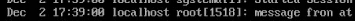
\includegraphics{17.png}
\end{enumerate}

\section{Контрольные вопросы}
\begin{enumerate}
	\item Как настроить задание \texttt{cron}, чтобы оно выполнялось раз в 2 недели? \\
	      \texttt{0 0 * * MON/1 cmd [arg...]} -- в данном случае, комманда будет выполнятся каждый второй понедельник в 00:00
	\item Как настроить задание \texttt{cron}, чтобы оно выполнялось 1-го и 15-го числа каждого месяца в 2 часа ночи? \\
	      \texttt{0 2 1,15 * * cmd [arg...]}
	\item Как настроить задание \texttt{cron}, чтобы оно выполнялось каждые 2 минуты каждый день? \\
	      \texttt{*/1 * * * * cmd [arg...]}
	\item Как настроить задание \texttt{cron}, чтобы оно выполнялось 19 сентября ежегодно? \\
	      \texttt{0 0 19 9 * cmd [arg...]}
	\item Как настроить задание \texttt{cron}, чтобы оно выполнялось каждый четверг сентября ежегодно? \\
	      \texttt{0 0 * 9 THU cmd [arg...]}
	\item Какая команда позволяет вам назначить задание \texttt{cron} для пользователя \texttt{alice}? Приведите подтверждающий пример. \\
	      \texttt{mm hh DD MM DW user cmd [arg...]} \\
	      \texttt{*/1 * * * * alice logger This message is written by alice each even minute}
	\item Как указать, что пользователю \texttt{bob} никогда не разрешено назначать задания через \texttt{cron}? Приведите подтверждающий пример. \\
	      Добавить имя пользователя \texttt{bob} в файл \texttt{/etc/cron.deny}
	\item Вам нужно убедиться, что задание выполняется каждый день, даже если сервер во время выполнения временно недоступен. Как это сделать? \\
	      Создать задание \texttt{cron} с необходимыми настройками времени
	\item Какая команда позволяет узнать, запланированы ли какие-либо задания на выполнение планировщиком \texttt{atd}? \\
	      \texttt{atq}
\end{enumerate}

\section{Вывод}
В ходе выполнения данной работы я получил навыков работы с планировщиками событий \texttt{cron} и \texttt{at}.

\end{document}
